%!TEX root = ../thesis.tex
%*******************************************************************************
%****************************** Second Chapter *********************************
%*******************************************************************************

\chapter{Marco teórico}

\ifpdf
    \graphicspath{{Chapter2/Figs/Raster/}{Chapter2/Figs/PDF/}{Chapter2/Figs/}}
\else
    \graphicspath{{Chapter2/Figs/Vector/}{Chapter2/Figs/}}
\fi


\section{Tecnologías}

\subsection{HTTP}

HTTP, Hypertext Transfer Protocol (Protocolo de Transferencia de Hipertexto) por sus
siglas, es el protocolo por el cual se comunican navegadores, servidores y aplicaciones
relacionadas con la web alrededor de todo el mundo.

Este protocolo se encuentra en la capa de aplicación del modelo OSI. Ha estado en uso por
la World-Wide Web (WWW) desde 1990. Su primera versión hace referencia a HTTP/0.9 y era un 
protocolo simple para la transferencia de datos a través de la internet.

HTTP/1.0 surge a través de la definición del RFC 1945, este mejoró sustancialmente la
comunicación permitiendo a los mensajes encontrarse en formato MIME (Multipurpose
Internet Mail Extensions). Los servidores web adjuntan un tipo MIME a todas sus peticiones
HTTP. Cuando un navegador web obtiene una respuesta desde un servidor, mira el tipo MIME
asociado a ella para ver si sabe cómo manejar el archivo. La mayoría de los navegadores
pueden manejar cientos de tipos de archivos populares: Imágenes, videos, sonidos,
documentos de texto, entre otros.

La última versión de este procolo es la 2.0, definida en el RFC 7540 en el año 2015. Un
gran avance en esta última versión contribuye a disminuir el tráfico innecesario en 
la red definiendo un mapeo optimizado de la semántica de HTTP a una conexión subyacente.

El modo de funcionamiento es muy sencillo. Esta compuesto por dos partes quienes son 
las partes que se comunican, estas son el cliente y el servidor. Básicamente el cliente
envía peticiones al servidor y este debe servirlas en caso de poder. De lo contrario, 
el servidor devolverá el error correspondiente a alguna de las posibles causas. Algunas 
de las más comunes son que el recurso que el servidor busca no se encuentre, que el 
recurso no esté disponible, que se haya movido de lugar o que haya habido algún error 
interno.

\begin{figure}[htbp!] 
\centering    
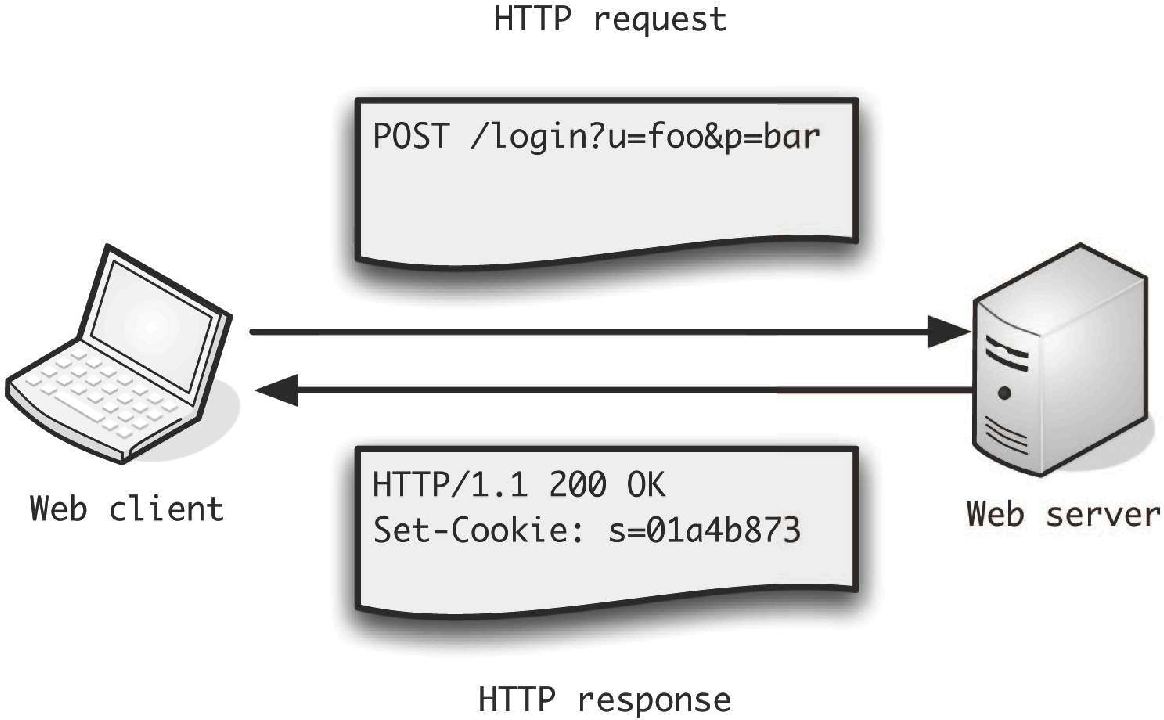
\includegraphics[width=0.5\textwidth]{http1}
\caption[HTTP]{Este es el comportamiento con información básica del protocolo HTTP}
\label{fig:http-behavior}
\end{figure}


\subsection{API REST}

\subsection{AJAX}

\subsection{JWT}

\subsection{Memoria Cache}


\section{Herramientas y tecnologías utilizadas}

\subsection{PHP}

\subsection{Lumen Framework}

\subsection{SQL}

\subsection{Taiga}

\subsection{Vagrant}

\subsection{Git}